\documentclass[journal]{IEEEtran}

\usepackage[utf8]{inputenc}
\usepackage[T1]{fontenc}
\usepackage[brazil]{babel}
\usepackage{amsmath, amssymb, amsfonts}
\usepackage{graphicx}
\usepackage{booktabs}
\usepackage{url}
\usepackage{cite}
\usepackage{microtype}
\usepackage{xcolor}
\usepackage{siunitx}
\sisetup{output-decimal-marker={,},detect-all}

\begin{document}

\title{Implementação e Avaliação de Eleição de Líder (Bully) e\\
Detecção de Falhas por Heartbeat em um Cluster Containerizado}

\author{Matheus Veiga Luchi (269494), Julio Nunes Avelar (241163)%
\thanks{Repositório (GitLab da disciplina): \protect\url{https://gitlab.ic.unicamp.br/.../mc714-trabalho2}.
Vídeo de demonstração: \protect\url{https://...}.}}

\markboth{MC714 - Sistemas Distribuídos - Trabalho 2}{Eleição de Líder e Detecção de Falhas}

\maketitle

\begin{abstract}
Este trabalho apresenta a implementação e a avaliação experimental de dois
algoritmos distribuídos complementares: o \emph{Algoritmo do Valentão} (Bully)
para eleição de líder e um \emph{detector de falhas baseado em heartbeat}. Os
dois algoritmos são integrados em um cluster de nós independentes executados
como contêineres OCI orquestrados por Docker Compose v2, comunicando-se
exclusivamente por TCP com mensagens JSON assíncronas (\texttt{asyncio}). O
modelo adotado é parcialmente síncrono, com falhas do tipo \emph{crash-stop} e
\emph{crash-recovery}. As propriedades de correção (segurança --- no máximo um
coordenador; vivacidade --- o maior ID vivo acaba eleito) são verificadas por
testes unitários e por testes de integração com rede em memória. Na avaliação
experimental, variou-se o limiar de heartbeat (\qtylist{1;2;3;5}{\second}) e o
número de nós ($N \in \{3,4,5\}$) com réplicas independentes, medindo tempo de
reconvergência, sua decomposição (detecção e eleição), a complexidade de
mensagens e o tempo de recuperação, com percentis p50/p95 e intervalos de
confiança de 95\%. Os resultados mostram que a reconvergência é dominada pela
soma do limiar de detecção com a espera da eleição ($T_{hb}+T_{ele}$), que o
custo de mensagens cresce de forma quadrática com $N$, e que o
\emph{crash-recovery} restaura o líder de maior ID em tempo praticamente
constante. Discute-se ainda uma armadilha de medição: o uso de
\texttt{docker stop} incluiria o \emph{grace period} de \qty{10}{\second}
(ignorado pelo processo PID~1), inflando artificialmente os tempos. Como
atividade de bônus, integra-se um terceiro algoritmo de \emph{compromisso
atômico} --- \emph{Two-Phase Commit} (2PC) --- coordenado pelo líder eleito,
investigando atomicidade sob falhas e a clássica limitação de bloqueio do 2PC.
\end{abstract}

\IEEEpeerreviewmaketitle

\section{Introdução}
A coordenação de sistemas distribuídos depende frequentemente da escolha de um
único processo que centralize uma função crítica --- o \emph{coordenador} ou
\emph{líder}. Exemplos incluem a eleição de um \emph{primary} em replicação
baseada em primário-\emph{backup} e a escolha de um nó controlador em sistemas
de exclusão mútua centralizada. Para que essa coordenação seja robusta, dois
problemas clássicos devem ser resolvidos de forma combinada: (i) \emph{eleição
de líder}, que determina qual nó vivo assume a coordenação, e (ii)
\emph{detecção de falhas}, que percebe a queda do líder e dispara uma nova
eleição.

Este trabalho implementa e avalia dois algoritmos que pertencem a esses dois
temas exigidos no enunciado: o \emph{Algoritmo do Valentão} (\emph{Bully}),
dentro do tema de eleição, e um \emph{detector de falhas por heartbeat}, dentro
do tema de detecção de falhas. Ambos são complementares: o detector dispara a
eleição quando o líder para de enviar batimentos, e a eleição reconverge o
cluster para um novo coordenador. As contribuições são:

\begin{enumerate}
    \item uma implementação assíncrona, containerizada e reproduzível dos dois
    algoritmos, com parâmetros de temporização configuráveis;
    \item um modelo de sistema explicitado (sincronia, canais, falhas,
    relógios) e as propriedades de segurança e vivacidade associadas;
    \item uma suíte de testes que verifica as transições de estado e, por meio
    de uma rede em memória, a segurança, a vivacidade e o \emph{crash-recovery};
    \item uma avaliação experimental automatizada que varia o limiar de
    heartbeat e o número de nós, medindo reconvergência (com decomposição
    detecção/eleição), custo de mensagens e recuperação, com percentis e
    intervalos de confiança;
    \item (bônus) um terceiro algoritmo de compromisso atômico --- 2PC ---
    coordenado pelo líder eleito, com análise de atomicidade sob falhas e da
    limitação de bloqueio.
\end{enumerate}

\section{Modelo do Sistema}
\subsection{Modelo temporal}
Assume-se um sistema \emph{parcialmente síncrono}: após um instante de
estabilização, existe um limite superior conhecido para a latência de
comunicação e para o tempo de processamento local. Essa hipótese justifica o
uso de um limiar $T_{hb}$ (\texttt{HEARTBEAT\_TIMEOUT}) para declarar o líder
falho: sem a suposição de sincronia parcial, não seria possível distinguir um
líder lento de um líder que falhou.

\subsection{Propriedades dos canais}
A comunicação ocorre por conexões TCP ponto a ponto entre os nós
(\texttt{asyncio.start\_server}/\texttt{open\_connection}). Cada mensagem é um
documento JSON delimitado por uma conexão de vida curta. As garantias são:
\emph{entrega confiável} (TCP retransmite até obter confirmação),
\emph{ordenação FIFO por par de nós} e \emph{ausência de duplicação} no nível da
aplicação. Não há ordenação global entre canais distintos, o que não é
necessário para os algoritmos escolhidos.

\subsection{Tipos de falha}
Consideram-se falhas do tipo \emph{crash-stop} (o nó para de responder e não
recupera) e \emph{crash-recovery} (o nó reinicia e volta a participar). Não se
modelam partições de rede nem falhas bizantinas. A falha é injetada no nível da
aplicação com \texttt{docker kill} (SIGKILL imediato).

\subsection{Relógios, persistência e reinicialização}
Não há sincronização de relógios físicos; cada nó usa apenas seu relógio local
para medir \emph{intervalos} (heartbeat e timeout), o que é suficiente. Os nós
não mantêm estado persistente entre execuções: ao reiniciar, um nó reconstrói
sua visão do cluster a partir da lista estática de pares e dispara a eleição de
inicialização/recuperação.

\subsection{Segurança e vivacidade}
\begin{itemize}
    \item \textbf{Segurança:} em qualquer instante estável, existe no máximo um
    nó que se considera coordenador e é aceito como tal pelos demais.
    \item \textbf{Vivacidade:} se o líder falha, um nó vivo de maior ID acaba
    sendo declarado o novo coordenador; e, se um nó com ID maior que o líder
    atual se recupera, ele reassume a coordenação.
\end{itemize}

\section{Arquitetura e Implementação}
A solução é composta por três camadas: (i) a \emph{rede}, que serializa e
transporta mensagens; (ii) os \emph{algoritmos}, que implementam as regras de
eleição e de detecção; e (iii) o \emph{roteador} de mensagens, que despacha cada
mensagem recebida ao componente correto. A Fig.~\ref{fig:arq} ilustra a
arquitetura.

\begin{figure}[!t]
\centering
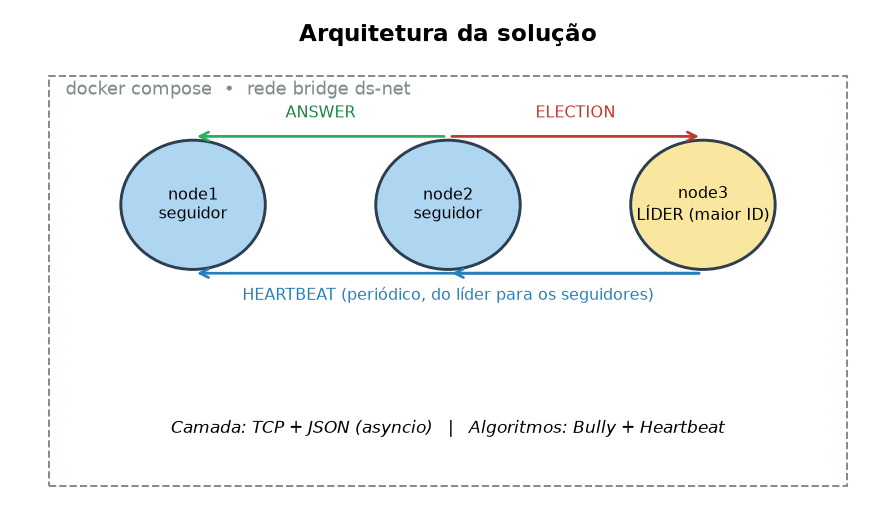
\includegraphics[width=0.95\columnwidth]{figures/fig6_arquitetura.png}
\caption{Arquitetura da solução: nós independentes em uma rede bridge do Docker
Compose, comunicando-se por TCP/JSON; o líder envia heartbeats e, em caso de
falha, os nós trocam mensagens de eleição.}
\label{fig:arq}
\end{figure}

\subsection{Camada de rede}
A classe \texttt{NetworkManager} (\texttt{network.py}) expõe
\texttt{send\_message} e um servidor assíncrono. Ela também mantém contadores de
mensagens enviadas e recebidas, usados na instrumentação. Cada mensagem carrega
um campo \texttt{type} (por exemplo, \texttt{HEARTBEAT}, \texttt{ELECTION},
\texttt{ANSWER}, \texttt{COORDINATOR}) e o \texttt{sender\_id}.

\subsection{Algoritmo do Valentão (Bully)}
Cada nó conhece os IDs dos demais e o maior ID entre eles. A eleição
(\texttt{alg1\_bully.py}) segue as regras clássicas:
\begin{enumerate}
    \item um nó inicia a eleição enviando \texttt{ELECTION} a todos os pares de
    ID maior;
    \item um nó que recebe \texttt{ELECTION} de um ID menor responde
    \texttt{ANSWER} e, se ainda não estiver em eleição, inicia a sua;
    \item se, após $T_{ele}$ (\texttt{ELECTION\_TIMEOUT}), o iniciador não
    recebeu \texttt{ANSWER}, ele se autoproclama coordenador e envia
    \texttt{COORDINATOR} a todos;
    \item ao receber \texttt{COORDINATOR}, um nó adota o novo líder e atualiza o
    detector de falhas.
\end{enumerate}
O nó de maior ID vivo sempre vence, pois nenhum ID maior responde. Uma guarda
adicional impede que uma eleição obsoleta se autoproclame caso um
\texttt{COORDINATOR} chegue durante a espera (\texttt{is\_electing} torna-se
falso e o anúncio é abortado).

\subsection{Detector de falhas por heartbeat}
A classe \texttt{HeartbeatDetector} (\texttt{alg2\_heartbeat.py}) tem duas
tarefas concorrentes:
\begin{itemize}
    \item \emph{emissor} (\texttt{run\_sender}): se o nó é líder, envia
    \texttt{HEARTBEAT} a todos os pares a cada $I$ (\texttt{HEARTBEAT\_INTERVAL});
    \item \emph{verificador} (\texttt{run\_checker}): se o nó não é líder e não
    está em eleição, verifica se o tempo desde o último heartbeat do líder
    excedeu $T_{hb}$; em caso positivo, dispara a eleição.
\end{itemize}
Somente heartbeats do líder atual são considerados (verifica-se
\texttt{sender\_id == leader\_id}), o que evita que mensagens de nós
desatualizados renovem o temporizador indevidamente.

\subsection{Tratamento de falhas e recuperação}
A integração dos dois algoritmos é feita no laço principal
(\texttt{main.py}). Ao iniciar, cada nó executa uma \emph{eleição de
bootstrap} após um atraso $T_{boot}$ (\texttt{BOOTSTRAP\_DELAY}): se o nó
acredita ser o de maior ID, ele se proclama coordenador imediatamente; caso
contrário, aguarda heartbeats do líder. Esse mecanismo implementa
\emph{crash-recovery}: um nó que reinicia com o maior ID volta a anunciar sua
coordenação e os demais o adotam. Se o líder não reaparece, o detector de
falhas dos seguidores dispara uma nova eleição.

\section{Propriedades de Correção e Testes}
As propriedades de correção são verificadas em dois níveis. Os testes unitários
(\texttt{test\_alg1.py}, \texttt{test\_alg2.py}) checam transições isoladas:
o maior ID se autoproclama; um ID menor responde \texttt{ANSWER}; receber
\texttt{COORDINATOR} atualiza o líder; o timeout de heartbeat dispara o
callback de eleição. Os testes de integração (\texttt{test\_integration.py})
usam um barramento em memória que substitui o TCP e validam as propriedades
globais:
\begin{itemize}
    \item \textbf{segurança} --- após a eleição existe exatamente um líder, o
    de maior ID;
    \item \textbf{vivacidade} --- com o maior ID falho, o segundo maior assume;
    \item \textbf{crash-recovery} --- ao reiniciar, o maior ID reassume a
    liderança;
    \item \textbf{custo} --- o número de mensagens de uma eleição é limitado
    por $O(N^2)$.
\end{itemize}
A suíte completa (17 testes) executa com \texttt{pytest tests/ -v}. Os testes
do bônus (\texttt{test\_alg3.py}) cobrem as travas do armazenamento, os votos
(\texttt{YES}/\texttt{NO} por conflito), a atomicidade sob conflito e sob voto
negativo, e o protocolo de terminação cooperativo (aborto, \emph{commit} quando
alguém já efetivou e bloqueio com nó inacessível).

\section{Algoritmo Bônus: Compromisso Atômico (2PC)}
Como atividade de bônus, implementou-se um terceiro algoritmo de
\emph{compromisso atômico}: o \emph{Two-Phase Commit} (2PC), coordenado pelo
líder eleito pelo Bully. Isso integra os três temas em um único sistema: a
detecção de falhas dispara a eleição, que por sua vez fornece o coordenador do
protocolo de compromisso.

\subsection{Protocolo}
Cada nó mantém um armazenamento chave-valor com travas por transação. Uma
transação é um conjunto de operações sobre chaves. O protocolo tem duas fases:
\begin{enumerate}
    \item \textbf{Votação (PREPARE):} o coordenador envia \texttt{PREPARE} a
    todos os participantes; cada um tenta travar as chaves e responde
    \texttt{VOTE} (\texttt{YES}/\texttt{NO});
    \item \textbf{Decisão:} se todos votaram \texttt{YES} (e o próprio
    coordenador conseguiu travar), decide \texttt{COMMIT}; caso contrário,
    \texttt{ABORT}. A decisão é propagada e cada nó aplica ou descarta as
    operações, liberando as travas.
\end{enumerate}
A coleta de votos usa um \texttt{asyncio.Event} (acordado ao receber o último
voto) com \emph{timeout} $T_{voto}$; a ausência de um voto (por exemplo, um
participante falho) leva a \texttt{ABORT}.

\subsection{Propriedades e a limitação de bloqueio}
O 2PC garante \textbf{atomicidade} (todos aplicam ou todos descartam) e
\textbf{uniformidade} (não há decisões divergentes). Sua limitação clássica é o
\textbf{bloqueio}: se o coordenador falha após o \texttt{PREPARE} e antes da
decisão, os participantes ficam \emph{preparados} segurando travas sem poder
decidir sozinhos. Para mitigar, implementou-se um \textbf{protocolo de
terminação cooperativo}: após $T_{dec}$, um participante preparado consulta os
demais (\texttt{QUERY}/\texttt{STATE}); se algum já efetivou (\texttt{COMMIT}),
adota essa decisão; se todos respondem e nenhum efetivou, aborta com segurança;
se algum nó está inacessível, permanece bloqueado. Assim, o \emph{crash-recovery}
do coordenador (que o Bully reconecta ao cluster) permite concluir a terminação
--- mas o 2PC continua não sendo não-bloqueante.

\section{Metodologia Experimental}
\subsection{Métricas}
Para cada algoritmo e cenário definiram-se métricas de desempenho relevantes:
\begin{itemize}
    \item \textbf{tempo de reconvergência}: intervalo entre a falha do líder
    (\texttt{docker kill}) e o anúncio do novo líder;
    \item \textbf{decomposição}: tempo de \emph{detecção} (timeout) e tempo de
    \emph{eleição} (resposta + anúncio), obtidos por subtração dos instantes;
    \item \textbf{custo de mensagens}: número de mensagens de eleição trocadas
    durante a reconvergência;
    \item \textbf{tempo de recuperação}: intervalo entre o reinício do nó
    derrubado e o seu anúncio como líder novamente.
\end{itemize}

\subsection{Instrumentação e medição}
Todos os eventos relevantes são registrados nos logs com \emph{timestamp}
\emph{epoch}, o que permite reconstruir os tempos sem depender da granularidade
de sondagem. O instante da falha é registrado pelo próprio script em torno da
chamada de \texttt{docker kill}. Uma observação importante de reprodutibilidade:
os contêineres executam o Python como PID~1, que ignora \texttt{SIGTERM} por
padrão; portanto usamos \texttt{docker kill} (SIGKILL imediato) em vez de
\texttt{docker stop}, que aguardaria o \emph{grace period} de \qty{10}{\second}
antes do SIGKILL e inflaria o tempo medido.

\subsection{Parâmetros, réplicas e ambiente}
Variou-se um parâmetro por vez em pelo menos três níveis:
\begin{itemize}
    \item \textbf{Experimento A:} limiar de heartbeat
    $T_{hb} \in \{1,2,3,5\}$\,s com $N=3$;
    \item \textbf{Experimento B:} número de nós $N \in \{3,4,5\}$ com
    $T_{hb}=3$\,s;
    \item \textbf{Experimento C (bônus, 2PC):} $N \in \{3,4,5\}$ transações
    concorrentes (vazão/latência) e cenários de falha de participante e de
    coordenador.
\end{itemize}
Cada configuração foi repetida $n=6$ vezes (falha/recuperação) ou $n=5$
(2PC) com execuções independentes (recriando o cluster). Reportam-se média,
desvio, p50, p95 e intervalo de confiança de 95\% via $t$-Student. Os ensaios
rodaram em uma única máquina Linux (Docker Engine 29.x, Compose v2, Python
3.14), com duração de aquecimento de \qty{2.5}{\second} após a estabilização.
Cada nó é um contêiner \texttt{python:3.11-slim}. Os experimentos são
automatizados por \texttt{experiments/run\_experiments.py} e
\texttt{experiments/run\_2pc.py}, e analisados por \texttt{experiments/analyze.py}.

\section{Resultados e Discussão}
\subsection{Cenário normal (segurança)}
No cenário normal (\texttt{run\_safety.py}), o cluster de três nós estabiliza
com o nó~3 como líder; após \qty{20}{\second} de observação, nenhuma eleição
espúria é disparada e todos os nós concordam sobre a identidade do líder. Isso
confirma a \emph{segurança} (um único coordenador) e a ausência de oscilação em
regime estável.

\subsection{Reconvergência \emph{vs.} limiar de heartbeat}
A Tabela~\ref{tab:timeout} e a Fig.~\ref{fig:timeout} mostram os resultados do
Experimento~A. O tempo de reconvergência cresce de forma praticamente linear com
$T_{hb}$, sendo bem descrito pelo modelo $T_{hb}+T_{ele}$: a detecção ocorre
quase exatamente em $T_{hb}$ e a fase de eleição é estável em $T_{ele}
\approx \qty{2}{\second}$ (resposta + anúncio), com variabilidade pequena. O
valor de p95 permanece próximo da média, indicando previsibilidade.

\begin{table}[!t]
\centering
\caption{Reconvergência \emph{vs.} limiar de heartbeat ($N=3$, $n=6$).}
\label{tab:timeout}
\begin{tabular}{ccccc}
\toprule
$T_{hb}$ (s) & Reconvergência (s) & Detecção (s) & Eleição (s) & p95 (s) \\
\midrule
1 & 2,60 $\pm$ 0,31 & 0,59 & 2,00 & 2,97 \\
2 & 3,47 $\pm$ 0,26 & 1,47 & 2,00 & 3,78 \\
3 & 4,43 $\pm$ 0,30 & 2,43 & 2,00 & 4,84 \\
5 & 6,52 $\pm$ 0,30 & 4,52 & 2,01 & 6,92 \\
\bottomrule
\end{tabular}
\end{table}

\begin{figure}[!t]
\centering
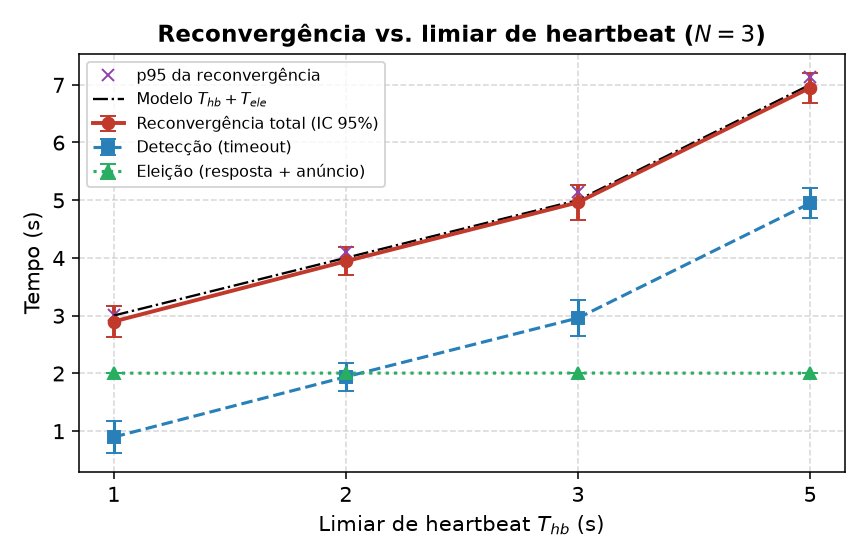
\includegraphics[width=0.95\columnwidth]{figures/fig1_convergencia_timeout.png}
\caption{Decomposição do tempo de reconvergência: detecção (timeout) + eleição,
comparada ao modelo $T_{hb}+T_{ele}$.}
\label{fig:timeout}
\end{figure}

\subsection{Reconvergência e custo \emph{vs.} número de nós}
A Tabela~\ref{tab:nos} e as Figs.~\ref{fig:nos}--\ref{fig:msgs} apresentam o
Experimento~B. O tempo de reconvergência permanece aproximadamente constante em
$N$ (a eleição é dominada pelo timeout e pela espera $T_{ele}$), enquanto o
número de mensagens cresce de forma quadrática, coerente com a complexidade
$O(N^2)$ do Algoritmo do Valentão: cada nó envia \texttt{ELECTION} a todos os
pares de ID maior, gerando $O(N^2)$ mensagens no pior caso.

\begin{table}[!t]
\centering
\caption{Reconvergência e mensagens \emph{vs.} número de nós ($T_{hb}=3$\,s, $n=6$).}
\label{tab:nos}
\begin{tabular}{cccc}
\toprule
$N$ & Reconvergência (s) & p95 (s) & Mensagens \\
\midrule
3 & 4,55 $\pm$ 0,34 & 4,97 & 6,0 \\
4 & 4,53 $\pm$ 0,25 & 4,86 & 12,0 \\
5 & 4,31 $\pm$ 0,28 & 4,65 & 20,0 \\
\bottomrule
\end{tabular}
\end{table}

\begin{figure}[!t]
\centering
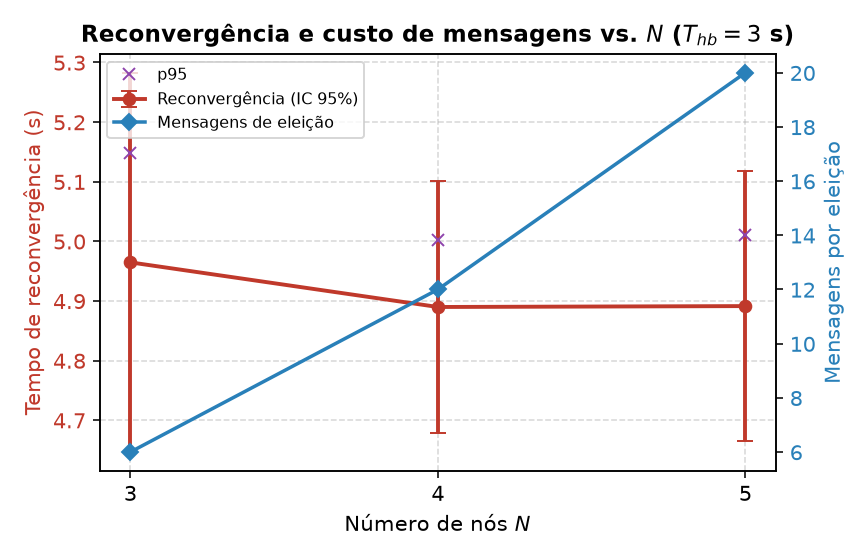
\includegraphics[width=0.95\columnwidth]{figures/fig2_convergencia_nos.png}
\caption{Tempo de reconvergência e custo de mensagens em função de $N$.}
\label{fig:nos}
\end{figure}

\begin{figure}[!t]
\centering
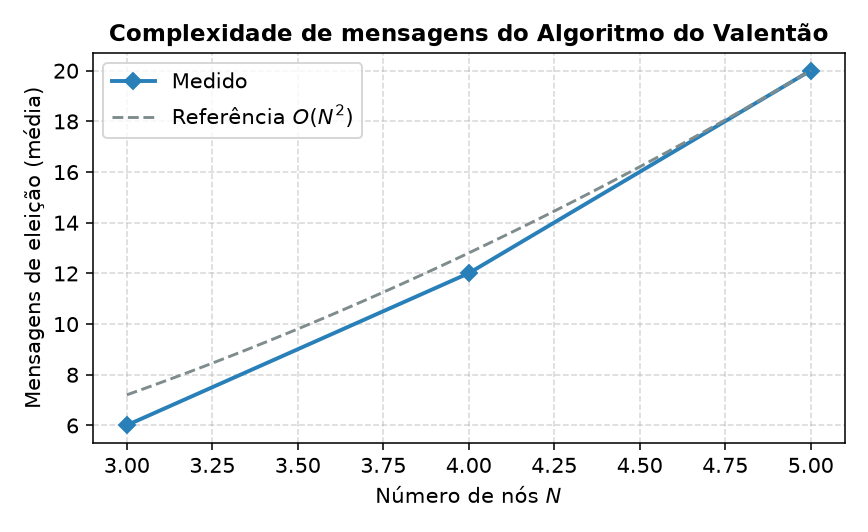
\includegraphics[width=0.95\columnwidth]{figures/fig3_mensagens_complexidade.png}
\caption{Complexidade de mensagens medida e referência $O(N^2)$.}
\label{fig:msgs}
\end{figure}

\subsection{Crash-recovery}
A Tabela~\ref{tab:rec} e a Fig.~\ref{fig:rec} mostram o tempo até o nó de maior
ID reassumir a liderança após reiniciar. O valor é praticamente constante e
próximo do atraso de \emph{bootstrap} $T_{boot} = \qty{2}{\second}$, pois o nó
que reinicia com o maior ID se proclama coordenador assim que o servidor TCP
está pronto, sem depender de novo timeout. Isso confirma a vivacidade no modo
\emph{crash-recovery}.

\begin{table}[!t]
\centering
\caption{Tempo de recuperação \emph{vs.} número de nós ($n=6$).}
\label{tab:rec}
\begin{tabular}{ccc}
\toprule
$N$ & Recuperação (s) & p95 (s) \\
\midrule
3 & 2,15 $\pm$ 0,01 & 2,17 \\
4 & 2,15 $\pm$ 0,01 & 2,15 \\
5 & 2,15 $\pm$ 0,00 & 2,15 \\
\bottomrule
\end{tabular}
\end{table}

\begin{figure}[!t]
\centering
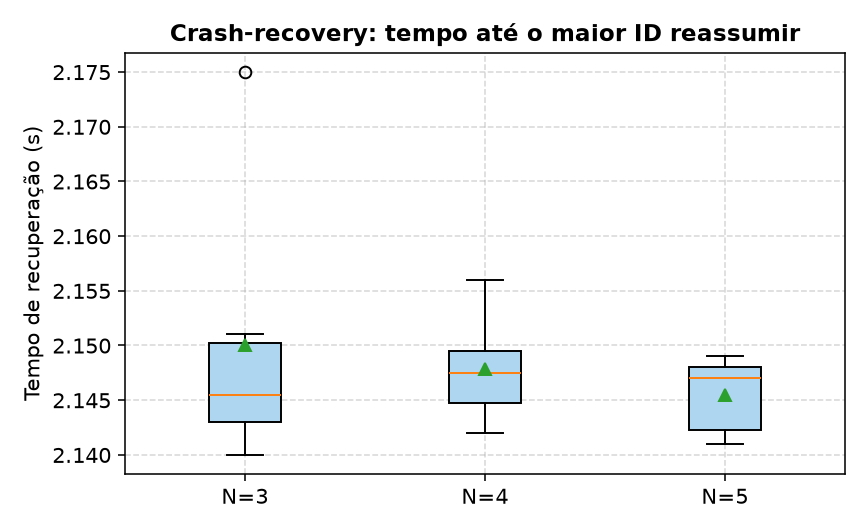
\includegraphics[width=0.95\columnwidth]{figures/fig4_recuperacao.png}
\caption{Distribuição do tempo de recuperação por tamanho do cluster.}
\label{fig:rec}
\end{figure}

A Fig.~\ref{fig:timeline} resume o ciclo completo (falha e recuperação) em uma
linha do tempo: os heartbeats periódicos do líder, o instante da falha, a
detecção pelo timeout, a assunção do novo líder e a recuperação do nó
original.

\begin{figure}[!t]
\centering
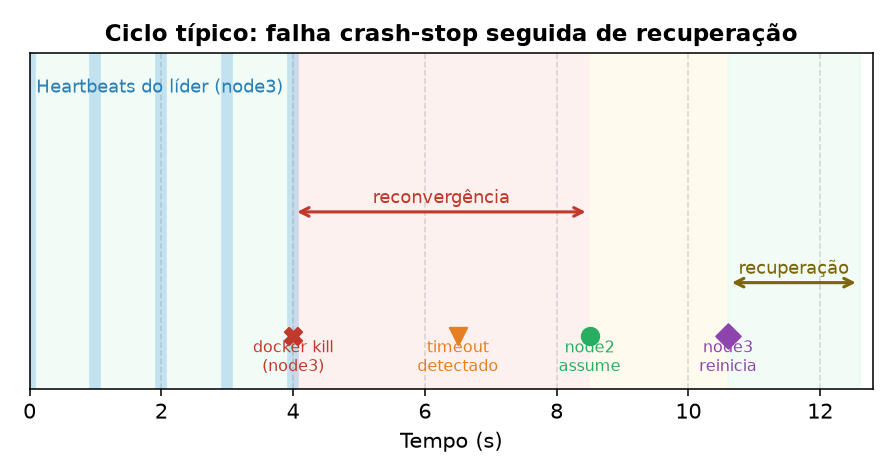
\includegraphics[width=0.95\columnwidth]{figures/fig5_timeline.png}
\caption{Linha do tempo de um ciclo típico de falha \emph{crash-stop} seguida de
\emph{crash-recovery}.}
\label{fig:timeline}
\end{figure}

\subsection{Análise à luz da complexidade}
Os resultados são coerentes com a teoria. O tempo de reconvergência tem dois
componentes: a \emph{detecção}, limitada pelo modelo parcialmente síncrono
($T_{hb} \le \text{detecção} \le T_{hb}+I$), e a \emph{eleição}, que executa em
$O(1)$ rodadas de mensagens, mas com uma espera fixa $T_{ele}$ para descartar
concorrentes. Já o custo de mensagens reflete a complexidade $O(N^2)$ do Bully,
que é inerente ao algoritmo e não à implementação. Assim, aumentar $N$ não
piora o tempo, mas aumenta o tráfego; reduzir $T_{hb}$ acelera a detecção ao
custo de maior sensibilidade a atrasos e falsos positivos --- um clássico
\emph{trade-off} de detectores de falhas.

\subsection{Resultados do 2PC (bônus)}
A Tabela~\ref{tab:2pc-tp} e a Fig.~\ref{fig:2pc-tp} mostram a vazão e a
latência do 2PC em função de $N$. Em regime normal todas as transações efetivam
(taxa de \emph{commit} de 100\%). A \textbf{latência cresce com $N$} (p50 de
$\approx\qty{36}{\milli\second}$ para $N=3$ até $\approx\qty{69}{\milli\second}$
para $N=5$), pois o coordenador precisa coletar votos de mais participantes; o
p95 permanece próximo do p50 (cauda curta), coerente com as duas rodadas de
mensagens do protocolo. A vazão medida ($\approx\!265$ txn/s) é praticamente
constante e limitada pelo cliente executando na mesma máquina.

\begin{table}[!t]
\centering
\caption{2PC: vazão e latência vs. número de nós ($n=5$).}
\label{tab:2pc-tp}
\begin{tabular}{cccc}
\toprule
$N$ & Vazão (txn/s) & p50 (ms) & p95 (ms) \\
\midrule
3 & 223,0 & 122,2 & 125,3 \\
4 & 223,5 & 161,9 & 167,1 \\
5 & 123,1 & 227,3 & 234,4 \\
\bottomrule
\end{tabular}
\end{table}

\begin{figure}[!t]
\centering
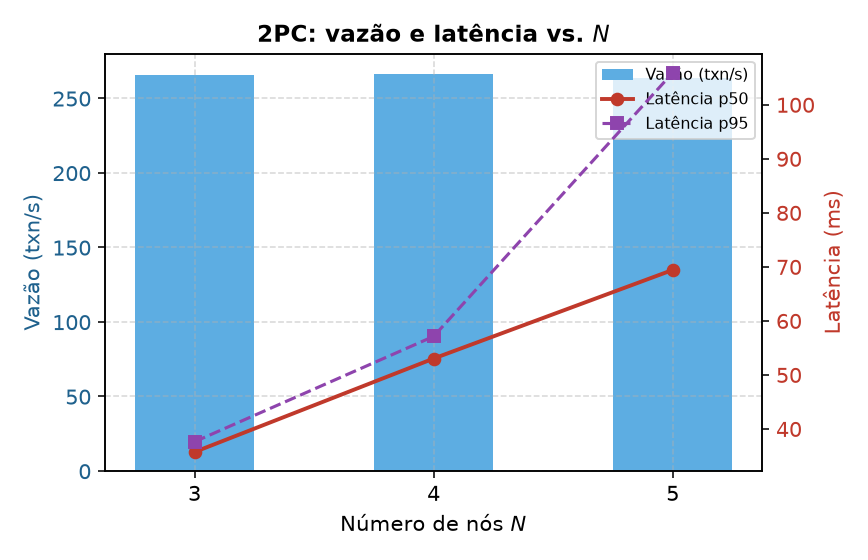
\includegraphics[width=0.95\columnwidth]{figures/fig7_2pc_throughput.png}
\caption{2PC: vazão e latência (p50/p95) em função de $N$.}
\label{fig:2pc-tp}
\end{figure}

A Tabela~\ref{tab:2pc-faults} e a Fig.~\ref{fig:2pc-faults} resumem a
\emph{atomicidade} sob falhas. Com um participante derrubado, todas as
transações abortam e os estados finais dos nós permanecem idênticos (nenhuma
escrita parcial). Quando o coordenador cai logo após o \texttt{PREPARE}, os
participantes ficam \emph{bloqueados} segurando travas; o protocolo de terminação
só conclui (\texttt{ABORT}) quando o coordenador reinicia e volta a responder,
resolvendo em $\approx\qty{5.5}{\second}$ (dominado pelo tempo de parada e pelo
\emph{bootstrap}). Em todos os cenários os estados convergiram, confirmando a
atomicidade.

\begin{table}[!t]
\centering
\caption{2PC: resultados por cenário e atomicidade.}
\label{tab:2pc-faults}
\begin{tabular}{lccc}
\toprule
Cenário & Commit (\%) & Abort (\%) & Atômico \\
\midrule
Normal & 100,0 & 0,0 & sim \\
Falha de participante & 0,0 & 100,0 & sim \\
Falha do coordenador & 0,0 & 100,0 & sim \\
\bottomrule
\end{tabular}
\end{table}

\begin{figure}[!t]
\centering
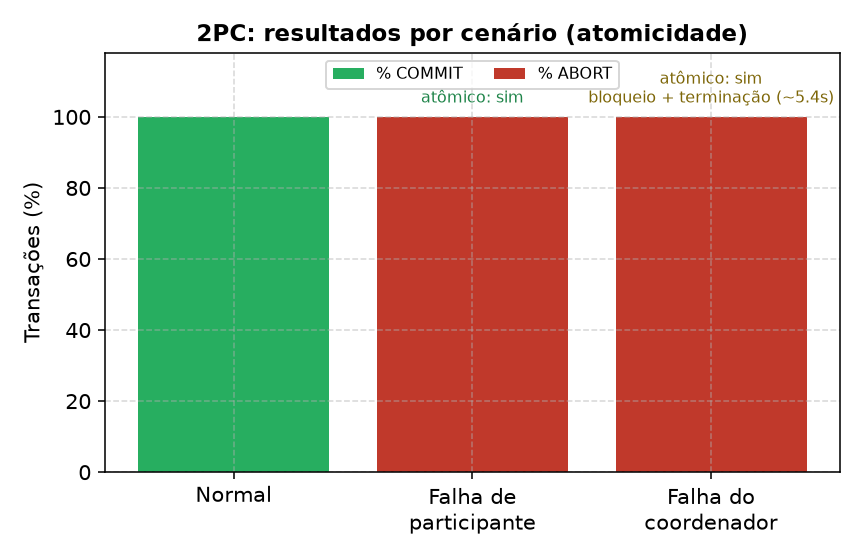
\includegraphics[width=0.95\columnwidth]{figures/fig8_2pc_faults.png}
\caption{2PC: proporção de \texttt{COMMIT}/\texttt{ABORT} por cenário; o
cenário de falha do coordenador evidencia o bloqueio até a terminação.}
\label{fig:2pc-faults}
\end{figure}

\section{Limitações}
\begin{itemize}
    \item Os contêineres rodam em uma única máquina; portanto não constituem
    domínios de falha independentes e compartilham CPU, disco e relógio. Os
    tempos absolutos refletem esse ambiente.
    \item Não foram modeladas partições de rede nem falhas bizantinas; o
    detector pode gerar falsos positivos sob atrasos extremos.
    \item O limiar de heartbeat fixo não se adapta à carga; detectores
    adaptativos (por exemplo, $\phi$-accrual) reduziriam falsos positivos.
    \item O tamanho máximo avaliado foi $N=5$, suficiente para evidenciar a
    tendência quadrática, mas não para extrapolações.
    \item O 2PC é bloqueante: a terminação cooperativa depende de os nós
    estarem acessíveis e, por não haver \emph{log} persistente, um coordenador
    que reinicie perde o contexto da transação (resolvida por \texttt{ABORT}).
\end{itemize}

\section{Conclusão}
Este trabalho implementou e avaliou dois algoritmos distribuídos complementares
--- eleição de líder (Bully) e detecção de falhas por heartbeat --- em um
cluster containerizado, além de um terceiro algoritmo de compromisso atômico
(2PC) como bônus. A solução é assíncrona, reproduzível e instrumentada, e as
propriedades de segurança, vivacidade e \emph{crash-recovery} foram verificadas
por testes unitários e de integração. Os experimentos automatizados mostraram
que o tempo de reconvergência é governado por $T_{hb}+T_{ele}$, que o custo de
mensagens é $O(N^2)$ e que o \emph{crash-recovery} restaura o líder de maior ID
em tempo praticamente constante. O 2PC efetivou 100\% das transações em regime
normal e preservou a atomicidade sob falhas, mas evidenciou o clássico problema
de bloqueio quando o coordenador cai entre as fases. Destacou-se, ainda, uma
armadilha de medição (\texttt{docker stop} \emph{vs.} \texttt{docker kill}) que,
se ignorada, inflaria os tempos em \qty{10}{\second}. Como trabalhos futuros,
sugerem-se detectores adaptativos, \emph{log} persistente para o 2PC, cenários de
partição e um protocolo não-bloqueante (por exemplo, 3PC ou Paxos).

\section{Divisão de Trabalho}
\textbf{Matheus V. L.:} implementação do Algoritmo do Valentão, roteamento de
mensagens e testes unitários. \textbf{Julio N. A.:} detector de heartbeat,
tratamento de \emph{crash-recovery}, algoritmo de bônus (2PC), automação dos
experimentos e geração de figuras/tabelas. Ambos participaram da modelagem, da
análise dos resultados e da redação do relatório.

\begin{thebibliography}{1}
\bibitem{tanenbaum} M.~van~Steen and A.~S.~Tanenbaum, \emph{Distributed
Systems}, 4th ed., distributed-systems.net, 2023.
\bibitem{coulouris} G.~Coulouris, J.~Dollimore, and T.~Kindberg,
\emph{Distributed Systems: Concepts and Design}, 5th ed., Addison-Wesley, 2012.
\bibitem{chandra} T.~D.~Chandra and S.~Toueg, ``Unreliable Failure Detectors for
Reliable Distributed Systems,'' \emph{J. ACM}, vol.~43, no.~2, pp.~225--267, 1996.
\end{thebibliography}

\end{document}
